%Iyy
\begin{figure}[ht!]
\centering
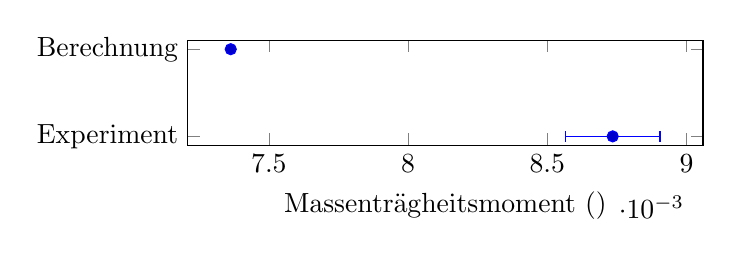
\begin{tikzpicture}
    \begin{axis}[
        try min ticks=2,
        width=.67\textwidth,
        height=.24\textwidth,
        %title = {Vergleich Startwerte und Endwerte: Amplitude},
        xlabel = {Massentr\"agheitsmoment ($\si{\kilo\gram\meter\squared}$)},
        symbolic y coords = {Experiment,Berechnung}
    ]
    \addplot+[
        only marks,error bars/.cd,
        x dir=both,x explicit,
        error bar style={line width=0.5pt},
        ]
    coordinates {
        (8.735e-3,Experiment) +- (170e-6,0)
        (7.363e-3,Berechnung)
    };
    \end{axis}
\end{tikzpicture}
\label{fig:pendel:results}
\end{figure}

%Ixx
\begin{figure}[ht!]
\centering
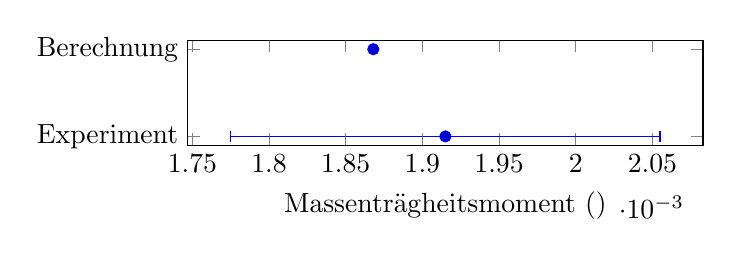
\begin{tikzpicture}
    \begin{axis}[
        try min ticks=2,
        width=.67\textwidth,
        height=.24\textwidth,
        %title = {Vergleich Startwerte und Endwerte: Amplitude},
        xlabel = {Massentr\"agheitsmoment ($\si{\kilo\gram\meter\squared}$)},
        symbolic y coords = {Experiment,Berechnung}
    ]
    \addplot+[
        only marks,error bars/.cd,
        x dir=both,x explicit,
        error bar style={line width=0.5pt},
        ]
    coordinates {
        (1.915e-3,Experiment) +- (140e-6,0)
        (1.868e-3,Berechnung)
    };
    \end{axis}
\end{tikzpicture}
\label{fig:pendel:results}
\end{figure}

%Izz
\begin{figure}[ht!]
\centering
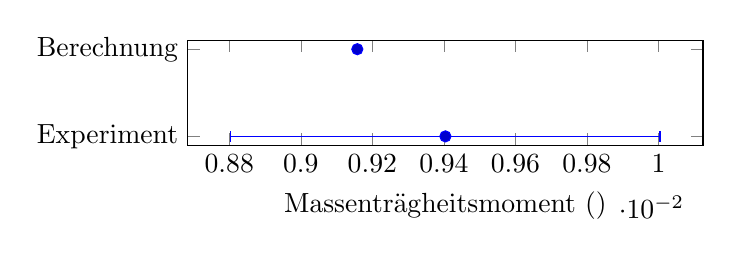
\begin{tikzpicture}
    \begin{axis}[
        try min ticks=2,
        width=.67\textwidth,
        height=.24\textwidth,
        %title = {Vergleich Startwerte und Endwerte: Amplitude},
        xlabel = {Massentr\"agheitsmoment ($\si{\kilo\gram\meter\squared}$)},
        symbolic y coords = {Experiment,Berechnung}
    ]
    \addplot+[
        only marks,error bars/.cd,
        x dir=both,x explicit,
        error bar style={line width=0.5pt},
        ]
    coordinates {
        (9.4042e-3,Experiment) +- (600e-6,0)
        (9.158e-3,Berechnung)
    };
    \end{axis}
\end{tikzpicture}
\label{fig:pendel:results}
\end{figure}

%15deg
\begin{figure}[ht!]
\centering
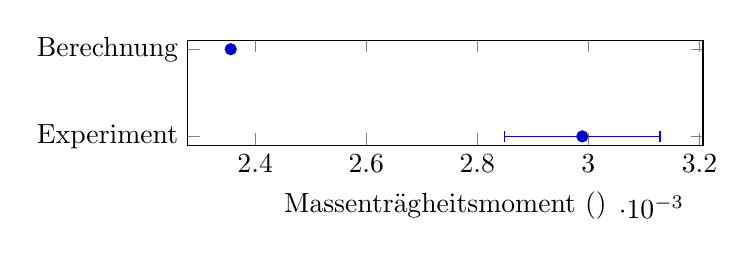
\begin{tikzpicture}
    \begin{axis}[
        try min ticks=2,
        width=.67\textwidth,
        height=.24\textwidth,
        %title = {Vergleich Startwerte und Endwerte: Amplitude},
        xlabel = {Massentr\"agheitsmoment ($\si{\kilo\gram\meter\squared}$)},
        symbolic y coords = {Experiment,Berechnung}
    ]
    \addplot+[
        only marks,error bars/.cd,
        x dir=both,x explicit,
        error bar style={line width=0.5pt},
        ]
    coordinates {
        (2.989e-3,Experiment) +- (140e-6,0)
        (2.356e-3,Berechnung)
    };
    \end{axis}
\end{tikzpicture}
\label{fig:pendel:results}
\end{figure}

%30deg
\begin{figure}[ht!]
\centering
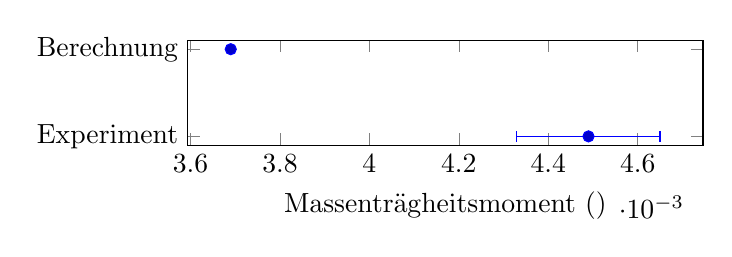
\begin{tikzpicture}
    \begin{axis}[
        try min ticks=2,
        width=.67\textwidth,
        height=.24\textwidth,
        %title = {Vergleich Startwerte und Endwerte: Amplitude},
        xlabel = {Massentr\"agheitsmoment ($\si{\kilo\gram\meter\squared}$)},
        symbolic y coords = {Experiment,Berechnung}
    ]
    \addplot+[
        only marks,error bars/.cd,
        x dir=both,x explicit,
        error bar style={line width=0.5pt},
        ]
    coordinates {
        (4.490e-3,Experiment) +- (160e-6,0)
        (3.69e-3,Berechnung)
    };
    \end{axis}
\end{tikzpicture}
\label{fig:pendel:results}
\end{figure}

%45deg
\begin{figure}[ht!]
\centering
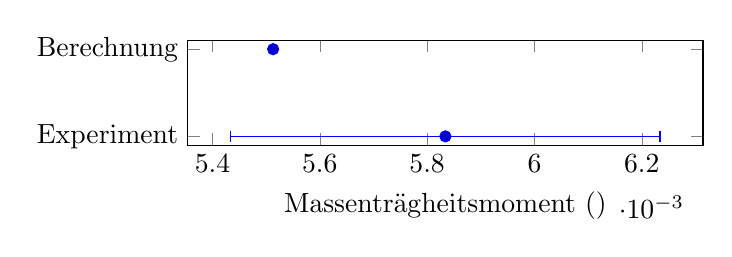
\begin{tikzpicture}
    \begin{axis}[
        try min ticks=2,
        width=.67\textwidth,
        height=.24\textwidth,
        %title = {Vergleich Startwerte und Endwerte: Amplitude},
        xlabel = {Massentr\"agheitsmoment ($\si{\kilo\gram\meter\squared}$)},
        symbolic y coords = {Experiment,Berechnung}
    ]
    \addplot+[
        only marks,error bars/.cd,
        x dir=both,x explicit,
        error bar style={line width=0.5pt},
        ]
    coordinates {
        (5.834e-3,Experiment) +- (400e-6,0)
        (5.513e-3,Berechnung)
    };
    \end{axis}
\end{tikzpicture}
\label{fig:pendel:results}
\end{figure}

%60deg
\begin{figure}[ht!]
\centering
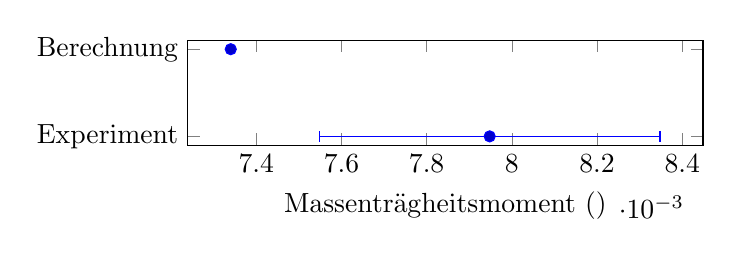
\begin{tikzpicture}
    \begin{axis}[
        try min ticks=2,
        width=.67\textwidth,
        height=.24\textwidth,
        %title = {Vergleich Startwerte und Endwerte: Amplitude},
        xlabel = {Massentr\"agheitsmoment ($\si{\kilo\gram\meter\squared}$)},
        symbolic y coords = {Experiment,Berechnung}
    ]
    \addplot+[
        only marks,error bars/.cd,
        x dir=both,x explicit,
        error bar style={line width=0.5pt},
        ]
    coordinates {
        (7.948e-3,Experiment) +- (400e-6,0)
        (7.340e-3,Berechnung)
    };
    \end{axis}
\end{tikzpicture}
\label{fig:pendel:results}
\end{figure}

%75deg
\begin{figure}[ht!]
\centering
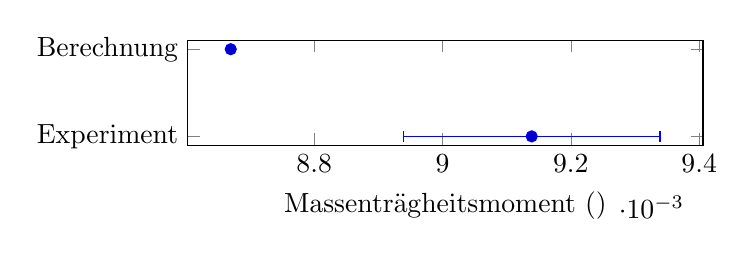
\begin{tikzpicture}
    \begin{axis}[
        try min ticks=2,
        width=.67\textwidth,
        height=.24\textwidth,
        %title = {Vergleich Startwerte und Endwerte: Amplitude},
        xlabel = {Massentr\"agheitsmoment ($\si{\kilo\gram\meter\squared}$)},
        symbolic y coords = {Experiment,Berechnung}
    ]
    \addplot+[
        only marks,error bars/.cd,
        x dir=both,x explicit,
        error bar style={line width=0.5pt},
        ]
    coordinates {
        (9.139e-3,Experiment) +- (200e-6,0)
        (8.670e-3,Berechnung)
    };
    \end{axis}
\end{tikzpicture}
\label{fig:pendel:results}
\end{figure}
